\chapter{Diseño\label{cap:disenho}}

En este capítulo se describe el diseño de la aplicación a desarrollar.
Tras analizar los requisitos especificados en el capítulo~\ref{cap:requisitos}, se ha decidido dividir la aplicación en dos partes, alojadas cada una en un servidor distinto: una interfaz web (\gls{front-end}) y un servicio web (\gls{back-end}).
Estos componentes están conectados por una red interna, y la comunicación entre ellos se realiza mediante llamadas  \gls{HTTP} (ver Figura~\ref{fig:arquitectura}).

\begin{figure}[!htp]
  \centering
  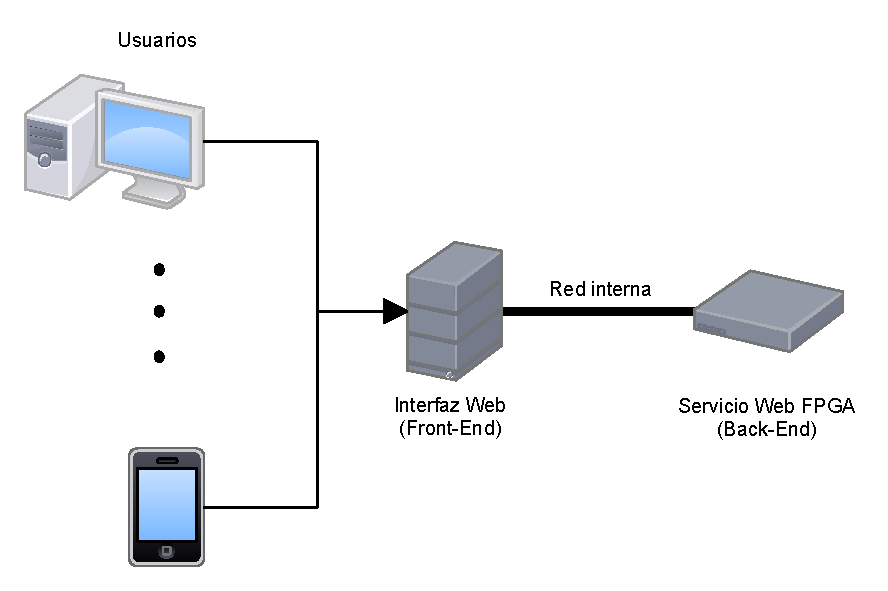
\includegraphics[width=0.7\textwidth,clip=true]{arquitectura}
  \caption{Arquitectura general de la aplicación.}
  \label{fig:arquitectura}
\end{figure}

La arquitectura propuesta tiene una serie de ventajas respecto a tener todos los elementos del sistema en un mismo servidor físico.
En primer lugar, se sobrecarga menos el servidor de la sonda de red, minimizando así el impacto que la aplicación pueda tener sobre el rendimiento de la captura y reproducción.
En segundo lugar, una división clara entre el \gls{back-end} y el \gls{front-end} facilita la adopción de tecnologías distintas en sendos componentes, utilizando en cada uno las que mejor se adapten al problema dado, y sin miedo a incompatibilidades (pues se comunican entre ellos por \gls{HTTP}, que es estándar).
En tercer lugar, se posibilita el gestionar desde un mismo \gls{front-end} distintas sondas de red que tengan instalado el mismo \gls{back-end}, sin que el usuario tenga que cambiar de plataforma.
Por último, al estar alojados en servidores distintos, la interfaz web podrá informar siempre al usuario del estado del sistema incluso cuando el servicio web no esté disponible.


\section{Back-End - Servicio Web FPGA\label{sec:dis:servicio_web_fpga}}

El componente \gls{back-end} se encarga de la interacción con la sonda de red (implementada en una \gls{FPGA}) y con el resto de partes involucradas en la reproducción y captura de tráfico de red.
Para ello, recibe peticiones \gls{HTTP} del \gls{front-end} (actuando en este caso como cliente), que se traducen en acciones sobre el sistema o en respuestas sobre el estado del mismo.
\begin{figure}[!htp]
  \centering
  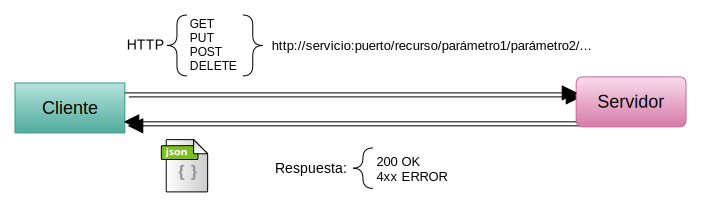
\includegraphics[width=0.95\textwidth,clip=true]{fpga_rest}
  \caption{Diagrama de flujo de un servicio \gls{REST}.}
  \label{fig:fpga_rest}
\end{figure}

La arquitectura de comunicación externa del \gls{back-end} se basa en el modelo de cliente-servidor \gls{REST} (ver Figura~\ref{fig:fpga_rest}).
Dentro de las directrices que marca este modelo, solo se han considerado útiles para el problema dado un subconjunto de ellas:
\begin{itemize}
  \item El protocolo entre el cliente y el servidor debe ser sin estado: cada mensaje \gls{HTTP} tiene que contener toda la información necesaria para comprender la petición.
  \item Las operaciones se aplican sobre recursos mediante llamadas a métodos \gls{HTTP}: \textit{GET} para obtener información sobre un recurso, \textit{POST}/\textit{PUT} para actualizarlos o crearlos y \textit{DELETE} para borrarlos.
  \item Cada recurso debe tener un identificador único (en este caso, una \gls{URL} única).
\end{itemize}

Se ha decidido no adoptar el resto de directrices \gls{REST} debido a que no encajaban dentro del modelo de funcionamiento de la aplicación.
Así, no se facilita el descubrimiento automático de recursos y métodos, ya que se ha considerado que no tiene sentido siendo éste un subsistema interno y no un componente público.
Por otra parte, no se permiten distintas representaciones de un mismo recurso, siendo \gls{JSON} la única representación utilizada.
No seguir estas directrices simplifica además la implementación del \gls{back-end}.

\begin{figure}[!htp]
  \centering
  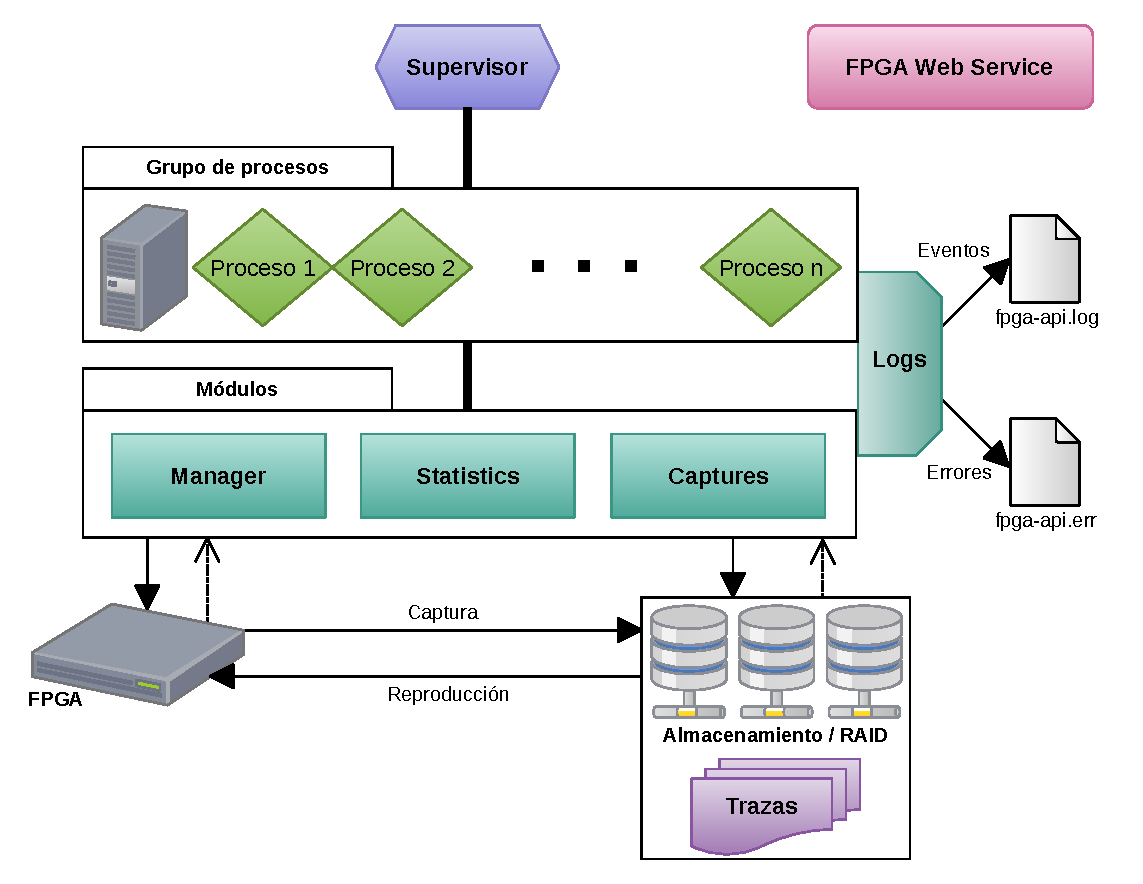
\includegraphics[width=0.95\textwidth,clip=true]{fpga}
  \caption{Arquitectura del \gls{servicioweb} \gls{FPGA}.}
  \label{fig:arquitectura_servicio}
\end{figure}

Internamente, el \gls{back-end} se estructura tal y como se describe en la Figura~\ref{fig:arquitectura_servicio}.
Un supervisor se encarga de vigilar al grupo de procesos que atienden las peticiones del \gls{front-end}, reemplazándolos en caso de que fallen.
Este grupo tiene tantos procesos como núcleos el servidor, adaptándose así a su arquitectura interna y consiguiendo por tanto una mayor disponibilidad y un menor tiempo de respuesta.
Por otro lado, con el objetivo de tener información detallada sobre el uso del servicio web, se registran todos los eventos y errores del \gls{back-end} en los \glspl{log} correspondientes.
Por último, se ha dividido el servicio web en tres módulos, cada uno con una funcionalidad asociada: \textit{manager}, \textit{captures} y \textit{statistics}.

\subsection{Manager\label{ssec:dis:manager}}

Este módulo se encarga de gestionar el estado de la sonda de red y del servidor que la aloja.
Permite por tanto instalar, programar y montar la sonda en modo reproducción o en modo captura, ordenarle reproducir o capturar tráfico y pararla.
Adicionalmente, maneja también otros aspectos del sistema, posibilitando reiniciar el servidor y formatear el sistema de almacenamiento en caso de ser necesario.


\subsection{Captures\label{ssec:dis:captures}}

Este módulo se ocupa de todos los aspectos relacionados con las \glspl{traza} de tráfico de red.
Permite así listar todas las \glspl{traza} disponibles, mostrando su nombre, fecha, tipo y tamaño.
Por otra parte, sobre una \gls{traza} concreta es capaz de detectar el formato interno de la misma, convertirla entre los formatos soportados, renombrarla o borrarla para liberar espacio de almacenamiento.


\subsection{Statistics\label{ssec:dis:statistics}}

Este módulo tiene como objetivo informar sobre el estado actual de la sonda de red, y proporcionar estadísticas sobre la reproducción o captura (en caso de existir una en curso).
Permite conocer además medidas sobre el almacenamiento: espacio ocupado, espacio disponible, velocidad de escritura global y por discos.


\section{Front-End - Interfaz web\label{sec:dis:interfaz_web}}

El \gls{front-end} se encarga de mostrar una interfaz web al usuario, recoger las acciones de éste y transformarlas en peticiones \gls{HTTP} al \gls{back-end}, informando de forma visual del resultado de la solicitud.
Este componente utiliza como punto de partida el \gls{framework} propio desarrollado (ver apéndice~\ref{extra:frameworkDesarrollado}).
Dicho \gls{framework} provee de una arquitectura y funcionalidad base a la interfaz, estructurando además los módulos de la misma siguiendo el patrón modelo-vista-controlador.

En el apartado visual, se ha decidido adoptar un diseño \textit{responsive}.
Esta filosofía de diseño se basa en la idea de que se debe adaptar la forma de mostrar una página para que la experiencia del usuario sea óptima independientemente del dispositivo que utilice (móvil, ordenador de sobremesa, etc.).
Para ello se utilizan una cuadrícula que cambia de posición y tamaño según sea el dispositivo desde el que se accede a la interfaz.
Ésta filosofía de diseño tiene una diferencia fundamental respecto al diseño \textit{adaptative}, que simplifica su implementación: mientras este último se basa en cargar distintos recursos de estilo según las características del dispositivo, el diseño \textit{responsive} utiliza una única cuadrícula que se ajusta en base a dichas características.

Respecto al idioma de la interfaz web, ésta estará disponible tanto en inglés como en español, pudiendo el usuario elegir el idioma que prefiera.
De forma similar, también se podrá seleccionar un tema visual para el \gls{front-end}.
Estos temas cambian el esquema de colores y aspectos menores de la interfaz gráfica.


\subsection{Maquetas\label{ssec:dis:maquetas}}

En este apartado se exponen las maquetas de las páginas principales de la interfaz, que sirven como guía para la implementación del \gls{front-end}.
Todas ellas cuentan con una barra superior de navegación, con enlaces al resto de pantallas principales de la interfaz.

En la Figura~\ref{fig:maqueta:configuracion} se muestra la maqueta de la pantalla de configuración de la aplicación.
En esta página se podrán configurar, mediante un formulario, la dirección del \gls{servicioweb} \gls{FPGA} (el \gls{back-end}), el idioma y el tema visual de la interfaz.
\begin{figure}[!htp]
  \centering
  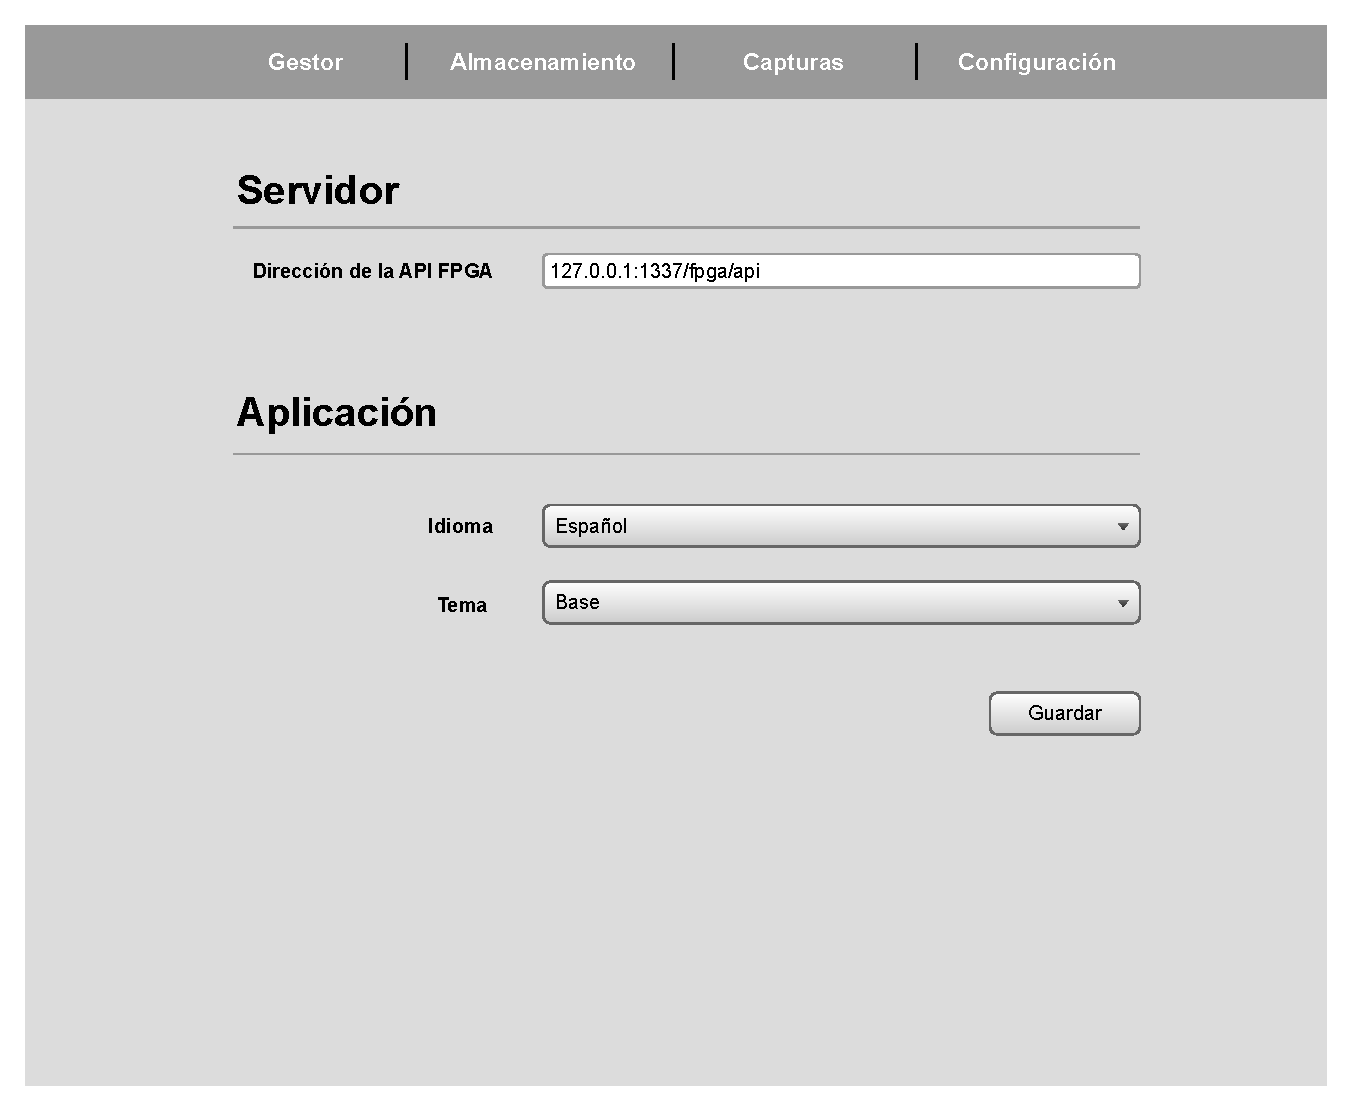
\includegraphics[width=\textwidth,clip=true]{maquetas/maqueta_configuracion}
  \caption{Maqueta de la pantalla de configuración de la aplicación.}
  \label{fig:maqueta:configuracion}
\end{figure}
\clearpage

En la Figura~\ref{fig:maqueta:almacenamiento} se muestra la maqueta de la pantalla de almacenamiento.
Esta página mostrará gráficas sobre el espacio disponible, y sobre estadísticas del \gls{RAID} en caso de estar configurado.
También se dará opción a formatear el \gls{RAID} en caso de que no tenga un rendimiento aceptable.
\begin{figure}[!htp]
  \centering
  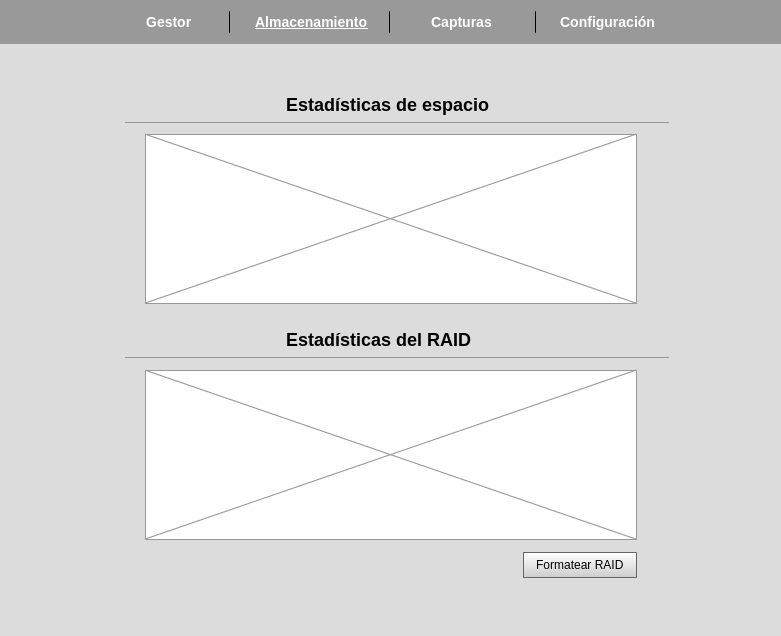
\includegraphics[width=\textwidth,clip=true]{maquetas/maqueta_almacenamiento}
  \caption{Maqueta de la pantalla de almacenamiento.}
  \label{fig:maqueta:almacenamiento}
\end{figure}
\clearpage

En la Figura~\ref{fig:maqueta:capturas} se muestra la maqueta de la pantalla de gestión de \glspl{traza}.
A la izquierda se podrán visualizar, en una tabla, todas las \glspl{traza} disponibles, con su nombre, tipo, tamaño y fecha.
Sobre esta tabla, una barra de acciones permitirá filtrar las \glspl{traza} según su tipo, o buscar alguna concreta por su nombre.
A la derecha se mostrará un panel con posibles acciones a realizar sobre la \gls{traza} seleccionada de la tabla: convertirla a otro formato, renombrarla o borrarla.
\begin{figure}[!htp]
  \centering
  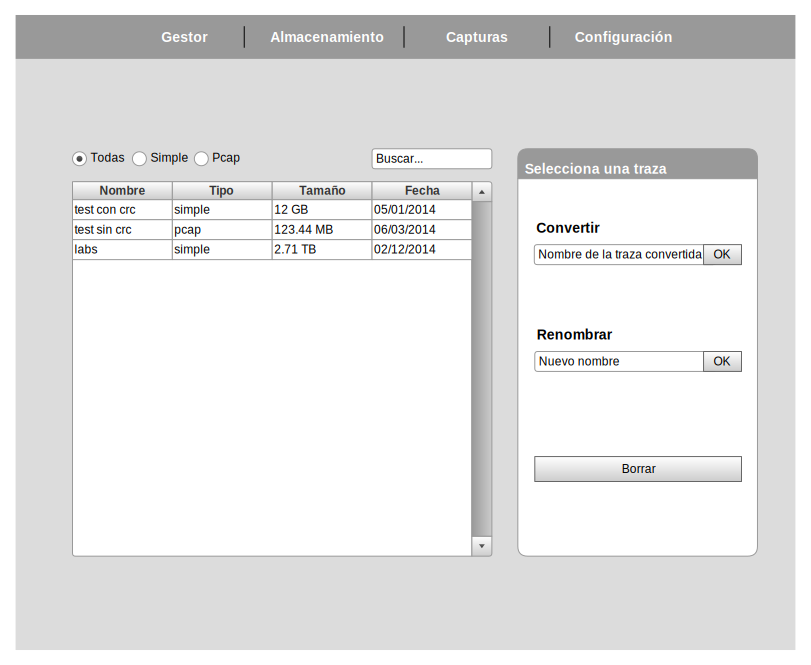
\includegraphics[width=\textwidth,clip=true]{maquetas/maqueta_capturas}
  \caption{Maqueta de la pantalla de gestión de \glspl{traza}.}
  \label{fig:maqueta:capturas}
\end{figure}
\clearpage

En la Figura~\ref{fig:maqueta:gestor_seleccion} se expone la maqueta de una de las pantallas de la página de gestión, que se mostrará en caso de que no se haya seleccionado aún ningún modo o cuando se quiera seleccionar otro.
Esta pantalla consta de dos botones, y pulsando alguno se inicializará la sonda en el modo correspondiente.
\begin{figure}[!htp]
  \centering
  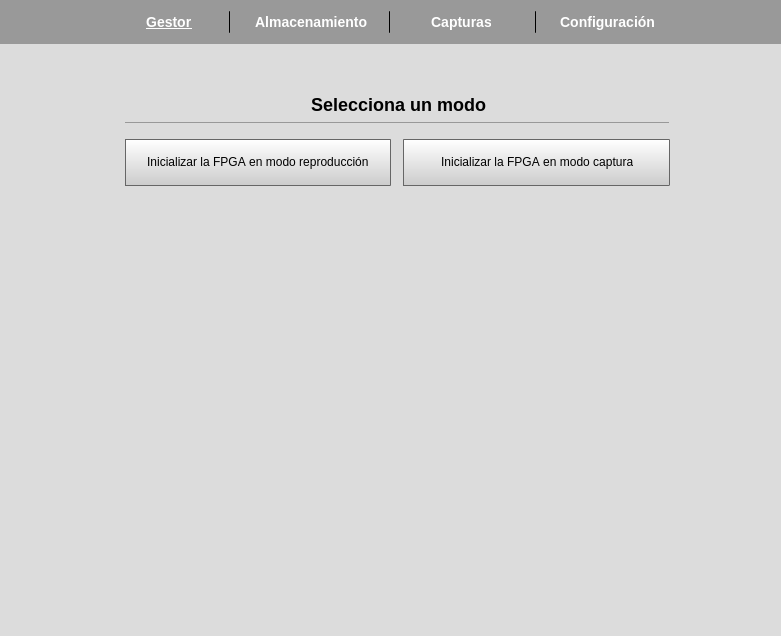
\includegraphics[width=\textwidth,clip=true]{maquetas/maqueta_gestor_seleccion}
  \caption{Maqueta de la pantalla de gestión - selección de modo.}
  \label{fig:maqueta:gestor_seleccion}
\end{figure}
\clearpage

En la Figura~\ref{fig:maqueta:gestor_capturador} se expone la maqueta de una de las pantallas de la página de gestión, que se mostrará cuando la sonda haya sido inicializada en modo captura.
En esta pantalla se podrá rellenar un formulario con el nombre de la \gls{traza} a capturar, su tamaño y el puerto del que capturar.
Pulsando el botón \textit{Capturar} se iniciará la captura de dicha \gls{traza}.
También se podrá volver a la página de selección de modo, pulsando el enlace inferior \textit{Cambiar de modo}.
\begin{figure}[!htp]
  \centering
  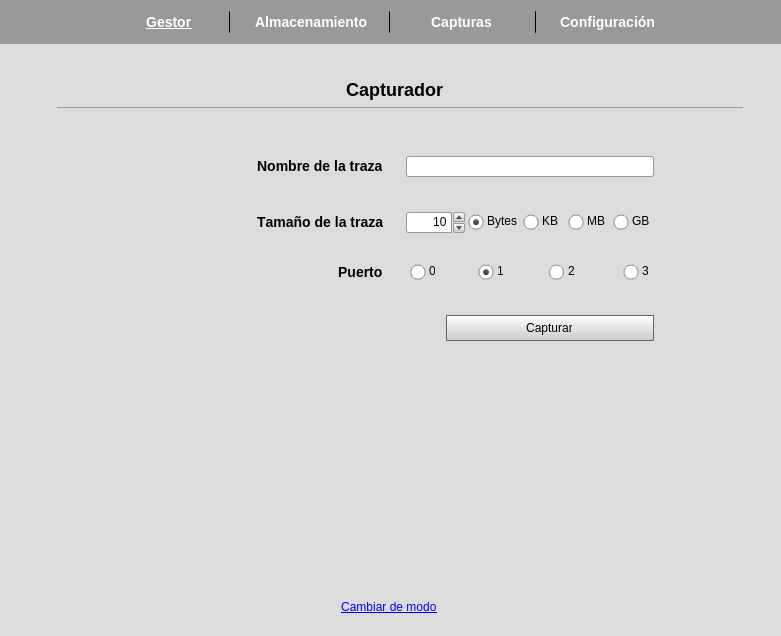
\includegraphics[width=\textwidth,clip=true]{maquetas/maqueta_gestor_capturador}
  \caption{Maqueta de la pantalla de gestión - formulario para capturar.}
  \label{fig:maqueta:gestor_capturador}
\end{figure}
\clearpage

En la Figura~\ref{fig:maqueta:gestor_capturando} se expone la maqueta de otra de las pantallas de gestión, que se mostrará cuando la sonda esté capturando tráfico de red.
En esta pantalla se podrán visualizar distintas estadísticas de la captura en curso, hasta que ésta finalice.
Adicionalmente, una barra de progreso indicará qué porcentaje de la \gls{traza} ha sido ya capturado.
También se podrá parar la captura, pulsando el botón \textit{Detener la captura}.
\begin{figure}[!htp]
  \centering
  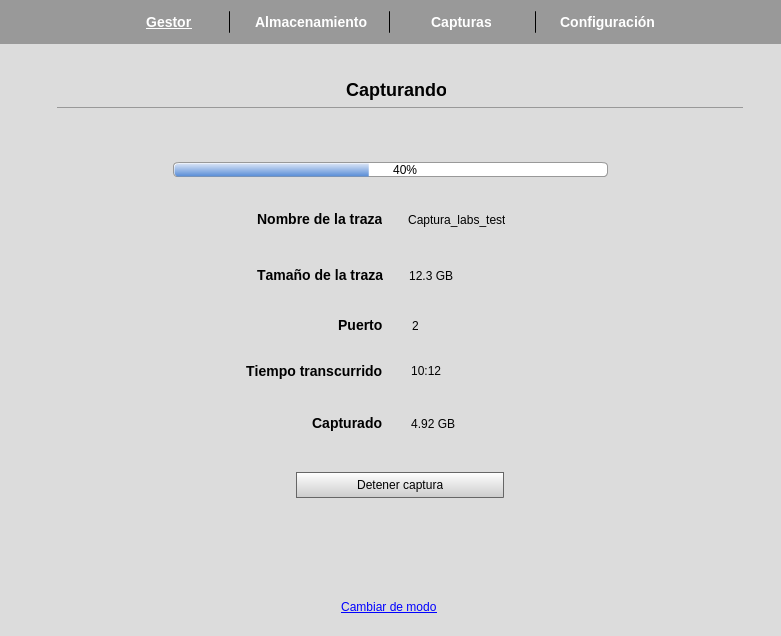
\includegraphics[width=\textwidth,clip=true]{maquetas/maqueta_gestor_capturando}
  \caption{Maqueta de la pantalla de gestión - capturando.}
  \label{fig:maqueta:gestor_capturando}
\end{figure}
\clearpage

En la Figura~\ref{fig:maqueta:gestor_reproductor} se expone la maqueta de otra de las pantallas de la página de gestión, que se mostrará cuando la sonda haya sido inicializada en modo reproducción.
A la izquierda se podrán visualizar, en una tabla, todas las \glspl{traza} disponibles para reproducir, con su nombre, tipo, tamaño y fecha.
Sobre esta tabla, una barra de acciones permitirá filtrar las \glspl{traza} según su tipo, o buscar alguna concreta por su nombre.
A la derecha se mostrará un panel con un formulario para configurar las opciones de reproducción: en bucle o no, \gls{IFG} y máscara de reproducción.
Pulsando el botón \textit{Reproducir} se iniciará la reproducción de la traza seleccionada.
También se podrá volver a la página de selección de modo, pulsando el enlace inferior \textit{Cambiar de modo}.
\begin{figure}[!htp]
  \centering
  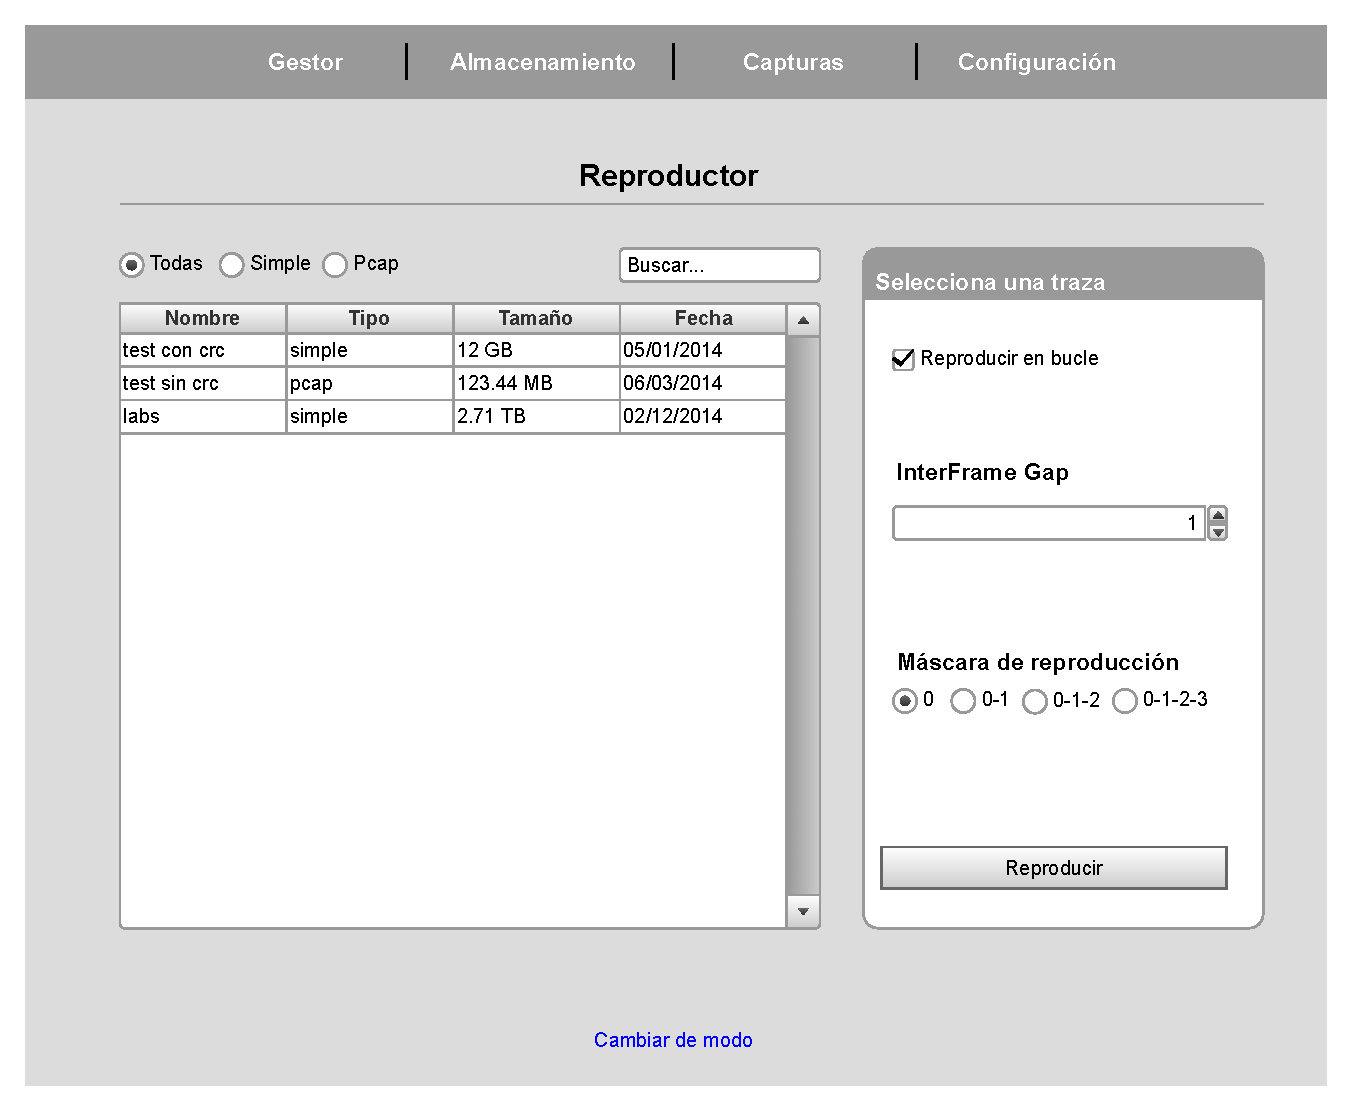
\includegraphics[width=\textwidth,clip=true]{maquetas/maqueta_gestor_reproductor}
  \caption{Maqueta de la pantalla de gestión - formulario para reproducir.}
  \label{fig:maqueta:gestor_reproductor}
\end{figure}
\clearpage

En la Figura~\ref{fig:maqueta:gestor_reproduciendo} se expone la maqueta de otra de las pantallas de gestión, que se mostrará cuando la sonda esté reproduciendo una \gls{traza}.
En esta pantalla se podrán visualizar distintas estadísticas de la reproducción en curso, hasta que ésta finalice.
También se podrá parar la reproducción, pulsando el botón \textit{Detener la reproducción}.
\begin{figure}[!htp]
  \centering
  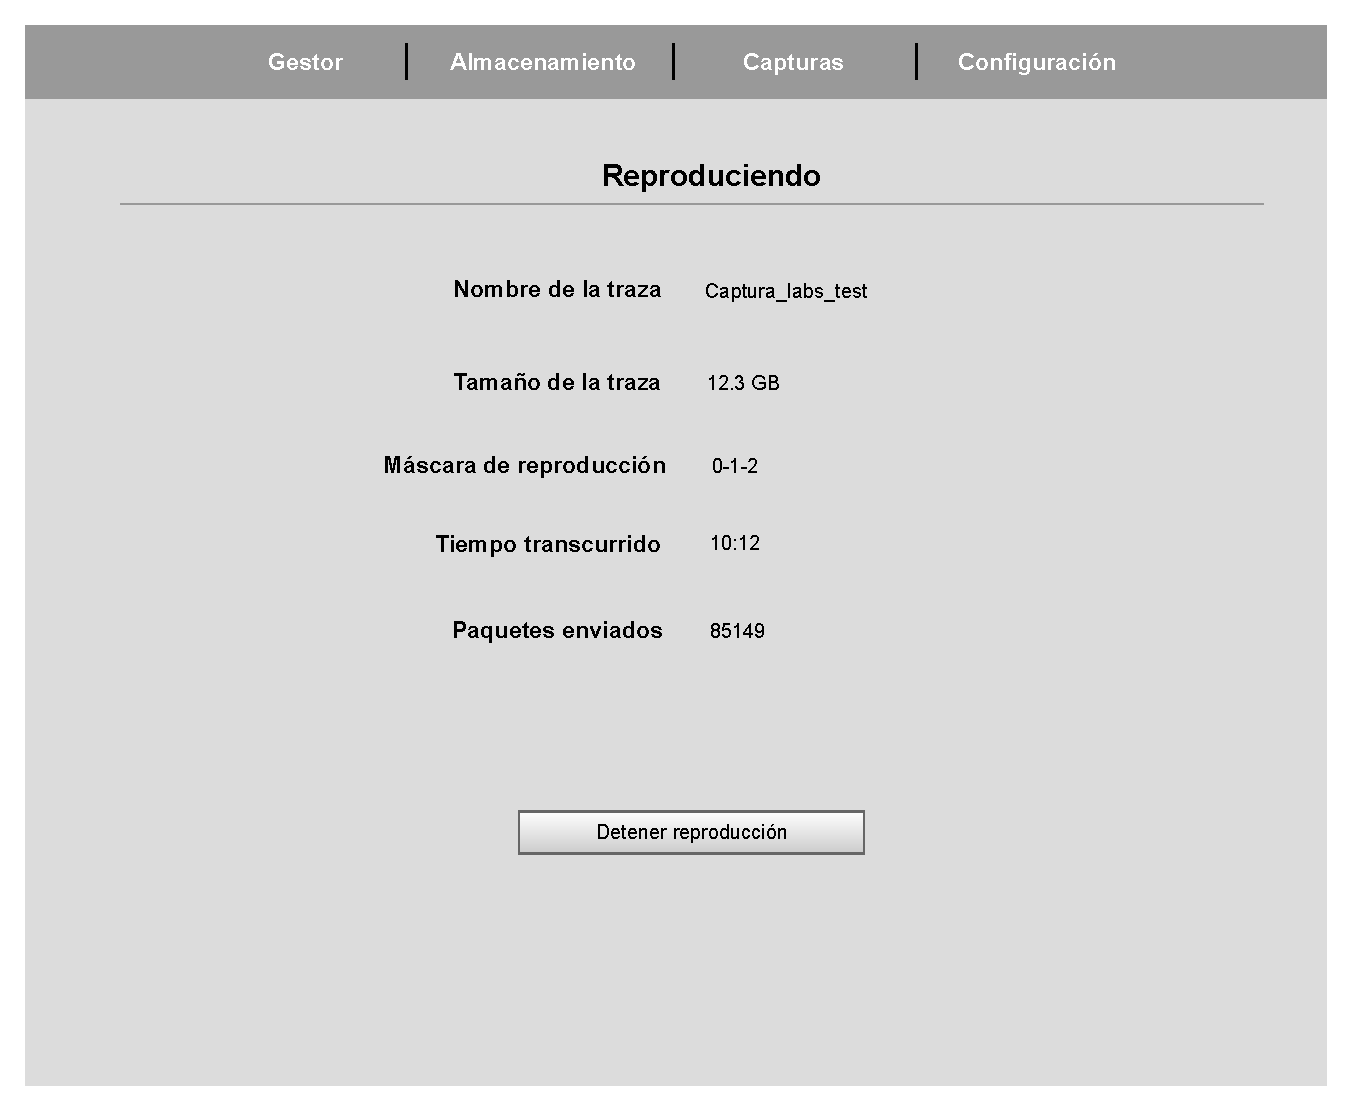
\includegraphics[width=\textwidth,clip=true]{maquetas/maqueta_gestor_reproduciendo}
  \caption{Maqueta de la pantalla de gestión - reproduciendo.}
  \label{fig:maqueta:gestor_reproduciendo}
\end{figure}
